\documentclass[light]{lutbeamer}

\usepackage{pgfpages}
\usepackage{ragged2e}
\usepackage{booktabs}
\usepackage{amssymb}
\usepackage{amsmath}
% \usepackage{enumitem} % Beamer ile çakıştığı için kaldırıldı
\usepackage{fontawesome5}
\usepackage{tikz}
\usepackage{pgfplots}
\pgfplotsset{compat=1.18}

% Beamer için enumerate stilini ayarla (a, b, c şeklinde)
\setbeamertemplate{enumerate item}{\alph{enumi})}

% ===================================================================
% METADATA
% ===================================================================
\setdepartment{OSTİM TEKNİK ÜNİVERSİTESİ}
\institute[Yazılım Mühendisliği]{YAZILIM MÜHENDİSLİĞİ BÖLÜMÜ}
\author{Dr.~Öğretim Üyesi Ufuk ASIL}
\title{Olasılık ve İstatistik}
\subtitle{Hafta 1: Bölüm 2 Alıştırmaları (2.1 -- 2.20) -- Detaylı Çözümlü}
\date{2025--2026 Bahar Dönemi}

\begin{document}

\setbeamertemplate{navigation symbols}{}
\maketitle{}

\section{Örnek Uzay (Sample Space)}

% ==================== SORU 2.1 ====================
\begin{frame}{Soru 2.1: Örnek Uzay Listeleme}
    Aşağıdaki örnek uzayların elemanlarını listeleyiniz:
    \begin{enumerate}
        \item 1 ile 50 arasındaki, 8 ile bölünebilen tamsayılar kümesi.
        \item $S = \{x \mid x^2 + 4x - 5 = 0\}$ kümesi.
        \item Bir madeni para, Yazı (T) gelene kadar veya üç kez Tura (H) gelene kadar atılıyor. Sonuçlar kümesi?
        \item $S = \{x \mid x \text{ bir kıtadır}\}$ kümesi.
        \item $S = \{x \mid 2x - 4 \geq 0 \text{ ve } x < 1\}$ kümesi.
    \end{enumerate}
\end{frame}

\begin{frame}[fragile]{Çözüm 2.1.a: 8 ile Bölünebilen Sayılar}
    \color{blue}
    \textbf{Soru:} 1 ile 50 arasındaki, 8 ile bölünebilen tamsayılar kümesi.
    
    \vspace{0.3cm}
    \textbf{Çözüm Adımları:}
    \begin{enumerate}
        \item 8'in katlarını bulmak için: $8 \times 1 = 8$, $8 \times 2 = 16$, \dots
        \item 50'yi geçmeyen en büyük kat: $8 \times 6 = 48$
        \item $8 \times 7 = 56 > 50$ (Dahil değil)
    \end{enumerate}
    
    \vspace{0.3cm}
    \begin{center}
    \fbox{$S = \{8, 16, 24, 32, 40, 48\}$}
    \end{center}
    
    \textbf{Kontrol:} 6 eleman var. Her biri 8'in katı ve 50'den küçük.
\end{frame}

\begin{frame}{Çözüm 2.1.b: İkinci Dereceden Denklem}
    \color{blue}
    \textbf{Soru:} $S = \{x \mid x^2 + 4x - 5 = 0\}$ kümesi.
    
    \vspace{0.3cm}
    \textbf{Çözüm Adımları:}
    \begin{enumerate}
        \item İkinci dereceden denklemi çözelim: $x^2 + 4x - 5 = 0$
        \item Çarpanlara ayırma yöntemi: $(x + 5)(x - 1) = 0$
        \item Kontrol: $(x+5)(x-1) = x^2 - x + 5x - 5 = x^2 + 4x - 5$ \checkmark
        \item Kökler: $x + 5 = 0 \Rightarrow x = -5$ veya $x - 1 = 0 \Rightarrow x = 1$
    \end{enumerate}
    
    \vspace{0.3cm}
    \begin{center}
    \fbox{$S = \{-5, 1\}$}
    \end{center}
\end{frame}

\begin{frame}{Çözüm 2.1.c: Para Atma Deneyi}
    \color{blue}
    \textbf{Soru:} Bir madeni para, Yazı (T) gelene kadar veya üç kez Tura (H) gelene kadar atılıyor.
    
    \vspace{0.3cm}
    \textbf{Durum Analizi:}
    \begin{itemize}
        \item \textbf{1. Atış T:} Deney biter $\rightarrow$ \{T\}
        \item \textbf{1. Atış H, 2. Atış T:} Deney biter $\rightarrow$ \{HT\}
        \item \textbf{İlk iki H, 3. Atış T:} Deney biter $\rightarrow$ \{HHT\}
        \item \textbf{Üç kez H:} 3 Tura geldi, deney biter $\rightarrow$ \{HHH\}
    \end{itemize}
    
    \vspace{0.3cm}
    \begin{center}
    \fbox{$S = \{T, HT, HHT, HHH\}$}
    \end{center}
    
    \textbf{Not:} 4 farklı sonuç var. Her durum deneyin bitiş koşulunu sağlar.
\end{frame}

\begin{frame}{Çözüm 2.1.d ve 2.1.e}
    \color{blue}
    \textbf{Soru d:} $S = \{x \mid x \text{ bir kıtadır}\}$
    
    \textbf{Çözüm:} Dünya'daki 7 kıta:
    \begin{center}
    \fbox{\parbox{0.9\textwidth}{$S = \{\text{Asya, Afrika, Kuzey Amerika, Güney Amerika,}$\\
    $\text{Avrupa, Avustralya, Antarktika}\}$}}
    \end{center}
    
    \vspace{0.5cm}
    \textbf{Soru e:} $S = \{x \mid 2x - 4 \geq 0 \text{ ve } x < 1\}$
    
    \textbf{Çözüm Adımları:}
    \begin{enumerate}
        \item İlk koşul: $2x - 4 \geq 0 \Rightarrow 2x \geq 4 \Rightarrow x \geq 2$
        \item İkinci koşul: $x < 1$
        \item Her iki koşul: $x \geq 2$ VE $x < 1$ $\Rightarrow$ Çelişki!
    \end{enumerate}
    
    \begin{center}
    \fbox{$S = \emptyset$ (Boş küme)}
    \end{center}
\end{frame}

% ==================== SORU 2.2 ====================
\begin{frame}{Soru 2.2: Kural Yöntemi ile Küme Tanımlama}
    Orijin merkezli ve yarıçapı 3 olan bir çemberin içindeki, birinci bölgedeki ($x>0, y>0$) noktaları içeren örnek uzay $S$'yi kural yöntemiyle tanımlayınız.
    
    \onslide<2->{
        \color{blue}
        \textbf{Çözüm:}
        
        \textbf{2.2:} $S = \{(x,y) \mid x^2 + y^2 < 9, x > 0, y > 0\}$
        
        \footnotesize
        \textbf{Not:} Eğer sınır (çember üzeri) dahil olsaydı: $x^2 + y^2 \leq 9$. Burada sadece ``iç bölge'' isteniyor
    }
\end{frame}

% ==================== SORU 2.3 ====================
\begin{frame}{Soru 2.3: Eşit Kümeler}
    Aşağıdaki olaylardan hangileri eşittir?
    \begin{enumerate}
        \item $A = \{1, 3\}$
        \item $B = \{x \mid x \text{ bir zardaki sayı}\}$
        \item $C = \{x \mid x^2 - 4x + 3 = 0\}$
        \item $D = \{x \mid x \text{ altı para atışındaki Tura sayısı}\}$
    \end{enumerate}
\end{frame}

\begin{frame}{Çözüm 2.3: Kümeleri Açalım}
    \color{blue}
    \textbf{Her Kümeyi Bulalım:}
    
    \begin{itemize}
        \item $A = \{1, 3\}$ (Doğrudan verilmiş)
        
        \item $B = \{x \mid x \text{ bir zardaki sayı}\} = \{1, 2, 3, 4, 5, 6\}$
        
        \item $C = \{x \mid x^2 - 4x + 3 = 0\}$
        
        Denklem: $(x-1)(x-3) = 0 \Rightarrow x = 1$ veya $x = 3$
        
        $\Rightarrow C = \{1, 3\}$
        
        \item $D = \{x \mid x \text{ altı para atışındaki Tura sayısı}\}$
        
        6 para atılırsa Tura sayısı: 0, 1, 2, 3, 4, 5 veya 6 olabilir
        
        $\Rightarrow D = \{0, 1, 2, 3, 4, 5, 6\}$
    \end{itemize}
    
    \vspace{0.3cm}
    \begin{center}
    \fbox{\textbf{Cevap: } $A = C$}
    \end{center}
\end{frame}

% ==================== SORU 2.4 ====================
\begin{frame}{Soru 2.4: Zar Çifti Deneyi}
    Bir deneyde biri yeşil, diğeri kırmızı iki zar atılıyor. $x$ yeşil zarın, $y$ kırmızı zarın sonucu olsun.
    \begin{enumerate}
        \item Örnek uzay $S$'yi $(x, y)$ elemanlarını listeleyerek yazınız.
        \item Örnek uzay $S$'yi kural yöntemiyle ifade ediniz.
    \end{enumerate}
\end{frame}

\begin{frame}{Çözüm 2.4.a: İki Zar - Listeleme}
    \color{blue}
    \textbf{Çözüm:}
    
    Her iki zar da 1'den 6'ya kadar değer alabilir. $x$ = yeşil zar, $y$ = kırmızı zar.
    
    \vspace{0.2cm}
    \footnotesize
    \begin{align*}
    S = \{ &(1,1), (1,2), (1,3), (1,4), (1,5), (1,6), \\
           &(2,1), (2,2), (2,3), (2,4), (2,5), (2,6), \\
           &(3,1), (3,2), (3,3), (3,4), (3,5), (3,6), \\
           &(4,1), (4,2), (4,3), (4,4), (4,5), (4,6), \\
           &(5,1), (5,2), (5,3), (5,4), (5,5), (5,6), \\
           &(6,1), (6,2), (6,3), (6,4), (6,5), (6,6) \}
    \end{align*}
    
    \textbf{Toplam:} $6 \times 6 = 36$ eleman
\end{frame}

\begin{frame}{Çözüm 2.4.b: Kural Yöntemi}
    \color{blue}
    \textbf{Çözüm:}
    
    Kümeyi matematiksel notasyon ile ifade edelim:
    
    \vspace{0.5cm}
    \begin{center}
    \fbox{$S = \{(x,y) \mid x \in \{1,2,3,4,5,6\}, \, y \in \{1,2,3,4,5,6\}\}$}
    \end{center}
    
    \vspace{0.5cm}
    \textbf{Alternatif:}
    \begin{center}
    $S = \{(x,y) \mid 1 \leq x \leq 6, \, 1 \leq y \leq 6, \, x,y \in \mathbb{Z}\}$
    \end{center}
    
    \vspace{0.3cm}
    \textbf{Açıklama:} $x$ ve $y$'nin her biri bağımsız olarak 1'den 6'ya kadar tamsayı değer alır.
\end{frame}

% ==================== SORU 2.5 ====================
\begin{frame}{Soru 2.5: Zar ve Para Deneyi}
    Bir deneyde önce bir zar atılıyor.
    \begin{itemize}
        \item Eğer zar \textbf{çift} gelirse, bir para \textbf{bir kez} atılıyor.
        \item Eğer zar \textbf{tek} gelirse, para \textbf{iki kez} atılıyor.
    \end{itemize}
    Notasyon: Örneğin $4H$ (Zar 4, Para Tura), $3HT$ (Zar 3, Para Tura, sonra Yazı).
    
    \textbf{İstem:} Örnek uzay $S$'nin 18 elemanını gösteren bir ağaç diyagramı çiziniz.
\end{frame}

\begin{frame}{Çözüm 2.5: Koşullu Para Atma - Çift Zarlar}
    \color{blue}
    \textbf{1. Durum: Zar çift gelirse (2, 4, 6)}
    
    Para \textbf{bir kez} atılır: H veya T
    
    \begin{center}
    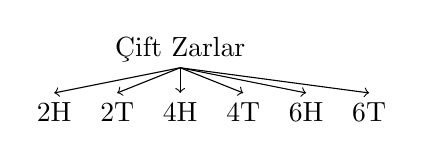
\begin{tikzpicture}[scale=0.8]
        \node at (0,0) {Çift Zarlar};
        \node at (-2,-1) {2H};
        \node at (-1,-1) {2T};
        \node at (0,-1) {4H};
        \node at (1,-1) {4T};
        \node at (2,-1) {6H};
        \node at (3,-1) {6T};
        
        \draw[->] (0,-0.3) -- (-2,-0.7);
        \draw[->] (0,-0.3) -- (-1,-0.7);
        \draw[->] (0,-0.3) -- (0,-0.7);
        \draw[->] (0,-0.3) -- (1,-0.7);
        \draw[->] (0,-0.3) -- (2,-0.7);
        \draw[->] (0,-0.3) -- (3,-0.7);
    \end{tikzpicture}
    \end{center}
    
    \textbf{Çift zarlar için:} $\{2H, 2T, 4H, 4T, 6H, 6T\}$ (6 eleman)
\end{frame}

\begin{frame}{Çözüm 2.5: Koşullu Para Atma - Tek Zarlar}
    \color{blue}
    \textbf{2. Durum: Zar tek gelirse (1, 3, 5)}
    
    Para \textbf{iki kez} atılır: HH, HT, TH, TT
    
    \footnotesize
    \begin{center}
    \begin{tabular}{ccl}
        Zar 1: & HH, HT, TH, TT & $\rightarrow$ \{1HH, 1HT, 1TH, 1TT\} \\
        Zar 3: & HH, HT, TH, TT & $\rightarrow$ \{3HH, 3HT, 3TH, 3TT\} \\
        Zar 5: & HH, HT, TH, TT & $\rightarrow$ \{5HH, 5HT, 5TH, 5TT\} \\
    \end{tabular}
    \end{center}
    
    \textbf{Tek zarlar için:} 12 eleman
    
    \vspace{0.5cm}
    \textbf{Toplam:} $6 + 12 = 18$ eleman
    
    \begin{center}
    \fbox{$S = \{2H, 2T, 4H, 4T, 6H, 6T, 1HH, 1HT, \ldots, 5TH, 5TT\}$}
    \end{center}
\end{frame}

% ==================== SORU 2.6 ====================
\begin{frame}{Soru 2.6: Jüri Seçimi}
    Bir cinayet davasında 4 yedek jüri arasından 2 kişi seçilecektir. $A_1A_3$, 1. ve 3. yedeğin seçilmesini göstersin. Örnek uzay $S$'nin 6 elemanını listeleyiniz.
\end{frame}

\begin{frame}{Çözüm 2.6: Kombinasyon ile Seçim}
    \color{blue}
    \textbf{Çözüm:}
    
    4 kişiden 2 kişi seçiyoruz. Sıra önemli değil (kombinasyon).
    
    \vspace{0.3cm}
    \textbf{Tüm İkili Seçimler:}
    \begin{itemize}
        \item $A_1$ ve $A_2$ seçilirse: $A_1A_2$
        \item $A_1$ ve $A_3$ seçilirse: $A_1A_3$
        \item $A_1$ ve $A_4$ seçilirse: $A_1A_4$
        \item $A_2$ ve $A_3$ seçilirse: $A_2A_3$
        \item $A_2$ ve $A_4$ seçilirse: $A_2A_4$
        \item $A_3$ ve $A_4$ seçilirse: $A_3A_4$
    \end{itemize}
    
    \vspace{0.3cm}
    \begin{center}
    \fbox{$S = \{A_1A_2, A_1A_3, A_1A_4, A_2A_3, A_2A_4, A_3A_4\}$}
    \end{center}
    
    \textbf{Kontrol:} $\binom{4}{2} = \frac{4!}{2!2!} = \frac{24}{4} = 6$ \checkmark
\end{frame}

% ==================== SORU 2.7 ====================
\begin{frame}{Soru 2.7: Öğrenci Sınıflandırması}
    Bir kimya sınıfından rastgele 4 öğrenci seçiliyor ve cinsiyetlerine göre (M: Erkek, F: Kadın) sınıflandırılıyor.
    \begin{itemize}
        \item $S_1$: Cinsiyet dizilimlerine göre örnek uzayı listeleyiniz.
        \item $S_2$: Seçilen kadın öğrenci sayısını temsil eden örnek uzayı tanımlayınız.
    \end{itemize}
\end{frame}

\begin{frame}{Çözüm 2.7.a: Cinsiyet Dizilimleri ($S_1$)}
    \color{blue}
    \textbf{Çözüm:}
    
    4 öğrenci var, her biri M veya F olabilir $\rightarrow$ $2^4 = 16$ durum
    
    \footnotesize
    \begin{align*}
    S_1 = \{ &MMMM, \, MMMF, \, MMFM, \, MMFF, \\
             &MFMM, \, MFMF, \, MFFM, \, MFFF, \\
             &FMMM, \, FMMF, \, FMFM, \, FMFF, \\
             &FFMM, \, FFMF, \, FFFM, \, FFFF \}
    \end{align*}
    
    \textbf{Açıklama:} İlk harf 1. öğrenci, son harf 4. öğrenciyi gösterir.
    Örnek: MFMM = (Erkek, Kadın, Erkek, Erkek)
\end{frame}

\begin{frame}{Çözüm 2.7.b: Kadın Sayısı ($S_2$)}
    \color{blue}
    \textbf{Çözüm:}
    
    4 öğrenci seçildiğinde, kadın sayısı 0'dan 4'e kadar olabilir:
    
    \begin{itemize}
        \item 0 kadın: MMMM
        \item 1 kadın: MMMF, MMFM, MFMM, FMMM (4 durum)
        \item 2 kadın: MMFF, MFMF, MFFM, FMMF, FMFM, FFMM (6 durum)
        \item 3 kadın: MFFF, FMFF, FFMF, FFFM (4 durum)
        \item 4 kadın: FFFF
    \end{itemize}
    
    \vspace{0.5cm}
    \begin{center}
    \fbox{$S_2 = \{0, 1, 2, 3, 4\}$}
    \end{center}
    
    \textbf{Not:} $S_2$, $S_1$'deki her durumu kadın sayısına göre özetler.
\end{frame}

\section{Olaylar (Events)}

% ==================== SORU 2.8 ====================
\begin{frame}{Soru 2.8: Zar Çifti Olayları}
    Soru 2.4'teki örnek uzay için (iki zar: yeşil $x$, kırmızı $y$):
    \begin{enumerate}
        \item $A$: Toplamın 8'den büyük olması.
        \item $B$: Herhangi bir zarda 2 gelmesi.
        \item $C$: Yeşil zarda 4'ten büyük bir sayı gelmesi.
        \item $A \cap C$
        \item $A \cap B$
        \item $B \cap C$
    \end{enumerate}
\end{frame}

\begin{frame}{Çözüm 2.8.a: Toplam > 8}
    \color{blue}
    \textbf{Olay A: } $x + y > 8$
    
    \vspace{0.3cm}
    \textbf{Sistematik Arama:}
    \begin{itemize}
        \item Toplam 9: (3,6), (4,5), (5,4), (6,3)
        \item Toplam 10: (4,6), (5,5), (6,4)
        \item Toplam 11: (5,6), (6,5)
        \item Toplam 12: (6,6)
    \end{itemize}
    
    \vspace{0.3cm}
    \begin{center}
    \fbox{\parbox{0.9\textwidth}{$A = \{(3,6), (4,5), (4,6), (5,4), (5,5), (5,6),$ \\ 
    $(6,3), (6,4), (6,5), (6,6)\}$}}
    \end{center}
    
    \textbf{Toplam:} 10 eleman
\end{frame}

\begin{frame}{Çözüm 2.8.b ve c: Zar 2 Gelme ve Yeşil > 4}
    \color{blue}
    \textbf{Olay B:} Herhangi bir zarda 2
    
    \textbf{Yeşil 2:} (2,1), (2,2), (2,3), (2,4), (2,5), (2,6) -- 6 eleman
    
    \textbf{Kırmızı 2:} (1,2), (3,2), (4,2), (5,2), (6,2) -- 5 eleman (2,2 tekrar edilmemeli)
    
    \begin{center}
    \fbox{\parbox{0.9\textwidth}{$B = \{(2,1), (2,2), (2,3), (2,4), (2,5), (2,6), (1,2), (3,2), (4,2), (5,2), (6,2)\}$}}
    \end{center}
    
    Toplam: 11 eleman
    
    \vspace{0.5cm}
    \textbf{Olay C:} Yeşil zar > 4 (yani $x \in \{5,6\}$)
    
    \begin{center}
    \fbox{$C = \{(5,1), (5,2), (5,3), (5,4), (5,5), (5,6), (6,1), \ldots, (6,6)\}$}
    \end{center}
    
    Toplam: 12 eleman ($2 \times 6 = 12$)
\end{frame}

\begin{frame}{Çözüm 2.8.d,e,f: Kesişimler}
    \color{blue}
    \textbf{d) $A \cap C$:} Toplam > 8 VE Yeşil > 4
    
    $A \cap C$'de $x \in \{5,6\}$ ve $x + y > 8$:
    \begin{center}
    \fbox{$A \cap C = \{(5,4), (5,5), (5,6), (6,3), (6,4), (6,5), (6,6)\}$}
    \end{center}
    
    \vspace{0.3cm}
    \textbf{e) $A \cap B$:} Toplam > 8 VE Bir zarda 2
    
    Eğer bir zar 2 ise, toplam en fazla $2 + 6 = 8$ olur. $8 > 8$ yanlış!
    \begin{center}
    \fbox{$A \cap B = \emptyset$}
    \end{center}
    
    \vspace{0.3cm}
    \textbf{f) $B \cap C$:} Bir zarda 2 VE Yeşil > 4
    
    Yeşil 5 veya 6, kırmızı 2:
    \begin{center}
    \fbox{$B \cap C = \{(5,2), (6,2)\}$}
    \end{center}
\end{frame}

% ==================== SORU 2.9 ====================
\begin{frame}{Soru 2.9: Zar ve Para Olayları}
    Soru 2.5'teki örnek uzay için:
    \begin{enumerate}
        \item $A$: Zarda 3'ten küçük bir sayı gelmesi.
        \item $B$: İki kez Yazı (TT) gelmesi.
        \item $A'$ (A'nın tümleyeni).
        \item $A' \cap B$
        \item $A \cup B$
    \end{enumerate}
\end{frame}

\begin{frame}{Çözüm 2.9.a,b: Olayları Bulma}
    \color{blue}
    \textbf{Hatırlatma:} $S = \{2H, 2T, 4H, 4T, 6H, 6T, 1HH, 1HT, 1TH, 1TT, \ldots\}$ (18 eleman)
    
    \vspace{0.3cm}
    \textbf{a) Olay A:} Zar < 3, yani zar 1 veya 2
    
    Zar 1 (tek, iki para): 1HH, 1HT, 1TH, 1TT
    
    Zar 2 (çift, bir para): 2H, 2T
    
    \begin{center}
    \fbox{$A = \{1HH, 1HT, 1TH, 1TT, 2H, 2T\}$} (6 eleman)
    \end{center}
    
    \vspace{0.3cm}
    \textbf{b) Olay B:} İki kez Yazı, yani TT
    
    Zar 1: 1TT, Zar 3: 3TT, Zar 5: 5TT
    
    \begin{center}
    \fbox{$B = \{1TT, 3TT, 5TT\}$} (3 eleman)
    \end{center}
\end{frame}

\begin{frame}{Çözüm 2.9.c,d,e: Tümleyen ve İşlemler}
    \color{blue}
    \textbf{c) $A'$:} $A$'nın tümleyeni = $S - A$
    
    $A = \{1HH, 1HT, 1TH, 1TT, 2H, 2T, \ldots\}$ (6 eleman)
    
    $S$'de olup $A$'da olmayanlar (yani Zar $\geq 3$):
    \begin{itemize}
        \item Zar 3: 3HH, 3HT, 3TH, 3TT
        \item Zar 4: 4H, 4T
        \item Zar 5: 5HH, 5HT, 5TH, 5TT
        \item Zar 6: 6H, 6T
    \end{itemize}
    (Toplam 12 eleman)
    
    \vspace{0.2cm}
    \textbf{d) $A' \cap B$:} Zar $\geq 3$ VE iki T
    
    $B$ içindekiler: 1TT, 3TT, 5TT. Bunlardan Zar $\geq 3$ olanlar:
    \begin{center}
    \fbox{$A' \cap B = \{3TT, 5TT\}$}
    \end{center}
    
    \vspace{0.2cm}
    \textbf{e) $A \cup B$:} $A$ veya $B$
    
    \begin{center}
    \fbox{$A \cup B = \{1HH, 1HT, 1TH, 1TT, 2H, 2T, 3TT, 5TT\}$}
    \end{center}
\end{frame}

% ==================== SORU 2.10 ====================
\begin{frame}{Soru 2.10: Su Kirliliği Testi}
    Üç nehirden örnek alınıyor ($F$: Güvenli, $N$: Güvenli Değil).
    \begin{enumerate}
        \item Örnek uzay $S$'yi listeleyiniz.
        \item $E$: En az iki nehrin güvenli olması olayını listeleyiniz.
        \item $\{ FFF, NFF, FFN, NFN \}$ kümesi hangi olayı tanımlar?
    \end{enumerate}
\end{frame}

\begin{frame}{Çözüm 2.10: Üç Nehir - Tüm Durumlar}
    \color{blue}
    \textbf{a) Örnek Uzay:}
    
    3 nehir var, her biri F veya N $\rightarrow$ $2^3 = 8$ durum
    
    \begin{center}
    \begin{tabular}{lll}
        Nehir 1 & Nehir 2 & Nehir 3 \\
        \hline
        F & F & F \\
        F & F & N \\
        F & N & F \\
        F & N & N \\
        N & F & F \\
        N & F & N \\
        N & N & F \\
        N & N & N \\
    \end{tabular}
    \end{center}
    
    \begin{center}
    \fbox{$S = \{FFF, FFN, FNF, FNN, NFF, NFN, NNF, NNN\}$}
    \end{center}
\end{frame}

\begin{frame}{Çözüm 2.10.b,c: Olayları Belirleme}
    \color{blue}
    \textbf{b) En az 2 nehir güvenli:}
    
    En az 2 F içeren durumlar:
    \begin{itemize}
        \item 3 F: FFF
        \item 2 F: FFN, FNF, NFF
    \end{itemize}
    
    \begin{center}
    \fbox{$E = \{FFF, FFN, FNF, NFF\}$} (4 eleman)
    \end{center}
    
    \vspace{0.5cm}
    \textbf{c) $\{FFF, NFF, FFN, NFN\}$ hangi olay?}
    
    \textbf{Analiz:} Verilen küme:
    \begin{itemize}
        \item FFF (2. nehir F)
        \item NFF (2. nehir F)
        \item FFN (2. nehir F)
        \item NFN (2. nehir F)
    \end{itemize}
    
    \textbf{Cevap:} ``İkinci nehir güvenlidir'' olayı.
    
    Matematiksel: $(N_2 = F)$
\end{frame}

% ==================== SORU 2.11 ====================
\begin{frame}{Soru 2.11: İş Başvurusu}
    \small
    İki pozisyon (Yrd. Doç. ve Öğretim Gör.) için başvuranlar: 2 Erkek ($M_1, M_2$), 2 Kadın ($F_1, F_2$).
    
    İlk pozisyon rastgele, ikinci pozisyon kalanlardan rastgele seçiliyor.
    \begin{enumerate}
        \item Örnek uzay $S$'yi listeleyiniz.
        \item $A$: Yrd. Doç. pozisyonunun bir erkek tarafından doldurulması.
        \item $B$: Tam olarak bir pozisyonun erkek tarafından doldurulması.
        \item $C$: Hiçbir pozisyonun erkek tarafından doldurulmaması.
        \item $A \cap B$, $A \cup C$ kümelerini bulunuz.
    \end{enumerate}
\end{frame}

\begin{frame}{Çözüm 2.11.a: Örnek Uzay - Tüm Seçimler}
    \color{blue}
    \textbf{Çözüm:}
    
    İlk seçim: 4 kişiden 1 $\rightarrow$ 4 seçenek
    
    İkinci seçim: Kalan 3 kişiden 1 $\rightarrow$ 3 seçenek
    
    Toplam: $4 \times 3 = 12$ seçim
    
    \vspace{0.3cm}
    \footnotesize
    \begin{center}
    \begin{tabular}{ll}
        $M_1$ seçilirse: & $M_1M_2, M_1F_1, M_1F_2$ \\
        $M_2$ seçilirse: & $M_2M_1, M_2F_1, M_2F_2$ \\
        $F_1$ seçilirse: & $F_1M_1, F_1M_2, F_1F_2$ \\
        $F_2$ seçilirse: & $F_2M_1, F_2M_2, F_2F_1$ \\
    \end{tabular}
    \end{center}
    
    \begin{center}
    \fbox{\parbox{0.9\textwidth}{$S = \{M_1M_2, M_1F_1, M_1F_2, M_2M_1, M_2F_1, M_2F_2,$ \\
    $F_1M_1, F_1M_2, F_1F_2, F_2M_1, F_2M_2, F_2F_1\}$}}
    \end{center}
\end{frame}

\begin{frame}{Çözüm 2.11.b,c,d: Olayları Belirleme}
    \color{blue}
    \footnotesize
    \textbf{b) Olay A: İlk pozisyon (Yrd. Doç.) erkek}
    
    İlk harf M: $\{M_1M_2, M_1F_1, M_1F_2, M_2M_1, M_2F_1, M_2F_2\}$ (6 eleman)
    
    \vspace{0.2cm}
    \textbf{c) Olay B: Tam olarak bir pozisyon erkek}
    
    (E,K) veya (K,E): $\{M_1F_1, M_1F_2, M_2F_1, M_2F_2, F_1M_1, F_1M_2, F_2M_1, F_2M_2\}$ (8)
    
    \vspace{0.2cm}
    \textbf{d) Olay C: Hiçbir pozisyon erkek değil}
    
    Her iki pozisyon kadın: $\{F_1F_2, F_2F_1\}$ (2 eleman)
    
    \vspace{0.3cm}
    \textbf{e) Kesişim ve Birleşim:}
    
    $A \cap B$: İlk erkek VE tam bir erkek = İlk erkek, ikinci kadın
    
    $A \cap B = \{M_1F_1, M_1F_2, M_2F_1, M_2F_2\}$ (4 eleman)
    
    \vspace{0.2cm}
    $A \cup C$: İlk erkek VEYA her ikisi kadın = $A + C$ (çünkü kesişimleri yok)
    
    $A \cup C = \{M_1M_2, M_1F_1, M_1F_2, M_2M_1, M_2F_1, M_2F_2, F_1F_2, F_2F_1\}$ (8)
\end{frame}

\section{Kümeler ve Venn Diyagramları}

% ==================== SORU 2.12 ====================
\begin{frame}{Soru 2.12: Diyet ve Egzersiz}
    Denek grupları:
    \begin{itemize}
        \item Grup 1: Hareketsiz ($Z$)
        \item Grup 2: Yürüyüş ($W$)
        \item Grup 3: Yüzme ($S$)
    \end{itemize}
    Her grubun yarısı Tuzsuz Diyet ($N$), diğer yarısı Tuzlu ($Y$).
    
    Ek Grup: İlaç tedavisi ($M$), Egzersiz/Diyet yok.
    
    \begin{enumerate}
        \item Örnek uzay $S$'yi listeleyiniz.
        \item $A$: İlaçsız denekler, $B$: Yürüyüşçüler. $A \cup B$ nedir?
        \item $A \cap B$ nedir?
    \end{enumerate}
\end{frame}

\begin{frame}{Çözüm 2.12: Gruplar ve Diyetler}
    \color{blue}
    \textbf{a) Örnek Uzay:}
    
    3 egzersiz grubu, her biri 2 diyet $\rightarrow$ $3 \times 2 = 6$ durum
    
    + 1 ilaç grubu (egzersiz yok, diyet yok)
    
    \begin{center}
    \fbox{$S = \{ZN, ZY, WN, WY, SN, SY, M\}$} (7 eleman)
    \end{center}
    
    \vspace{0.3cm}
    \textbf{b) $A \cup B$:}
    
    $A$ (İlaçsız) = $\{ZN, ZY, WN, WY, SN, SY\}$ (M hariç hepsi)
    
    $B$ (Yürüyüş) = $\{WN, WY\}$
    
    $A \cup B = A$ (Çünkü $B \subset A$)
    
    \textbf{c) $A \cap B$:}
    
    İlaçsız VE Yürüyüş = $\{WN, WY\}$
\end{frame}

% ==================== SORU 2.13, 2.14, 2.15, 2.16, 2.17, 2.18 ====================
\begin{frame}{Soru 2.13-2.18: Hızlı Geçiş}
    \color{blue}
    \small
    \textbf{2.13:} Venn diyagramı çiz (F: 4 kapı, S: Sunroof, P: Hidrolik) - 8 bölge
    
    \textbf{2.14:} Küme işlemleri: Verilen $S, A, B, C, D$ ile işlemler yapılacak
    
    \textbf{2.15:} Element kümeleri ile işlemler
    
    \textbf{2.16:} Aralık kümeleri: $M \cup N$, $M \cap N$, $M' \cap N'$
    
    \textbf{2.17:} Venn'de bölge tarama
    
    \textbf{2.18:} Ayrık olaylar: b) ve c) AYRIK
    
    \textit{(Bu soruların detaylı çözümleri için lütfen ders notlarına bakınız)}
\end{frame}

% ==================== SORU 2.19 ve 2.20 ====================
\begin{frame}{Soru 2.19 ve 2.20: Kamp Tatili - Venn Analizi}
    Bir ailenin tatili için olaylar:
    \begin{itemize}
        \item $M$: Mekanik sorun
        \item $T$: Trafik cezası
        \item $V$: Boş yer olmayan kamp alanı
    \end{itemize}
    
    Venn şemasında 8 bölge vardır.
    
    \textbf{Soru 2.19:} Bölgelerin anlamlarını söyleyiniz.
    
    \textbf{Soru 2.20:} Belirtilen olayların bölgelerini bulunuz.
\end{frame}

\begin{frame}{Çözüm 2.19 ve 2.20: Venn Bölgeleri}
    \color{blue}
    \footnotesize
    \textbf{Venn Şeması Bölgeleri:}
    \begin{enumerate}
        \item $M \cap T \cap V$ (Her üçü de)
        \item $M \cap T \cap V'$ (M ve T, V yok)
        \item $M \cap T' \cap V$ (M ve V, T yok)
        \item $M \cap T' \cap V'$ (Sadece M)
        \item $M' \cap T \cap V$ (T ve V, M yok)
        \item $M' \cap T \cap V'$ (Sadece T)
        \item $M' \cap T' \cap V$ (Sadece V)
        \item $M' \cap T' \cap V'$ (Hiçbiri)
    \end{enumerate}
    
    \textbf{2.20 Cevapları:}
    
    a) Bölge 7: $M' \cap T' \cap V$ (Sadece V var)
    
    b) Bölge 3: $M \cap T' \cap V$ (M ve V var, T yok)
    
    c) Bölge 3, 5, 7: $(M \cup V) \cap T'$ (M veya V var, T yok)
    
    d) Bölge 2, 4, 6, 8: $V'$ (V olmayan tüm bölgeler)
    
    \footnotesize
    \textbf{Kontrol:} $V'$ içinde V olan bölgeler (1,3,5,7) asla olamaz!
\end{frame}

\end{document}
